\textbf{See the instruction for questions \inteval{\value{question}+1} to \inteval{\value{question}+2}.}

\begin{center}
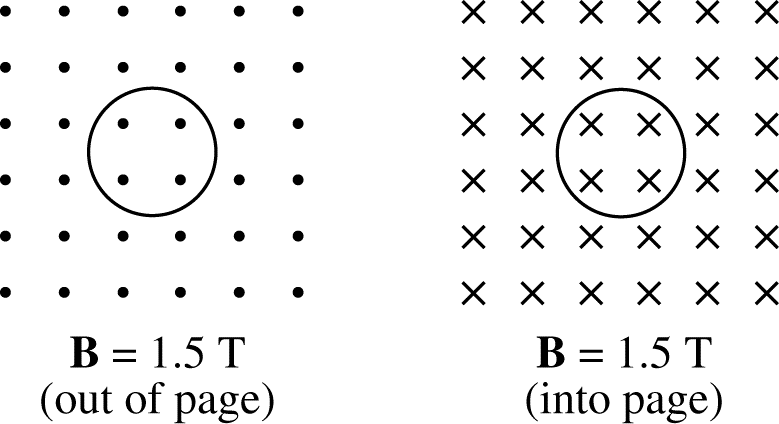
\includegraphics[scale=0.25]{images/img-012-025.png}
\end{center}

A circular conducting ring of area $0.20 \unit{m^2}$ lies in the plane of the page inside a spatially uniform magnetic field that is perpendicular to the page. The field changes smoothly from $1.5 \unit{T}$ directed out of the page, as shown above on the left, to $1.5 \unit{T}$ directed into the page, as shown above on the right. The change takes place at a constant rate during a total time interval of $0.6 \unit{s}$.

% Multiple Choice Question 26
\begin{questions}\setcounter{question}{25}\question
What is the magnitude of the average emf induced during the $0.6 \unit{s}$ time interval?

\begin{oneparchoices}
\choice $0 \unit{V}$
\choice $0.5 \unit{V}$
\choice $1.0 \unit{V}$
\choice $1.5 \unit{V}$
\choice $2.0 \unit{V}$
\end{oneparchoices}\end{questions}

% Multiple Choice Question 27
\begin{questions}\setcounter{question}{26}\question
When viewed as shown in the figure, what is the direction of the induced current during the first and second halves of the $0.6 \unit{s}$ time interval?

\tabto{0.75cm}\underline{First Half}
\tabto{8.00cm}\underline{Second Half}

\begin{choices}
\choice Clockwise                            \tabto{7.25cm} Clockwise
\choice Clockwise                            \tabto{7.25cm} Counterclockwise
\choice Counterclockwise                     \tabto{7.25cm} Clockwise
\choice Counterclockwise                     \tabto{7.25cm} Counterclockwise
\choice Undefined, since the current is zero \tabto{7.25cm} Undefined, since the current is zero
\end{choices}\end{questions}

